\documentclass[a4paper,11pt]{article}
\pdfoutput=1 % if your are submitting a pdflatex (i.e. if you have
             % images in pdf, png or jpg format)
\usepackage{color}
\usepackage{jcappub} % for details on the use of the package, please
                     %
\usepackage{amsmath}
\newcommand\ddfrac[2]{\frac{\displaystyle #1}{\displaystyle #2}}
\newcommand\ts{\mathcal{TS}}
\newcommand\tsbg{\mathcal{TS_{\mathrm{bg}}}}

\usepackage[T1]{fontenc} % if needed
\usepackage{threeparttable}
\usepackage[labelformat=empty]{subfig}
\usepackage{booktabs}
\usepackage{multirow}
\usepackage{placeins}
\usepackage[utf8]{inputenc}
\usepackage{indentfirst}
\usepackage[utf8]{inputenc}
\usepackage{tablefootnote}


\usepackage[dvipsnames]{xcolor}

\newcommand{\colorhref}[3][blue]{\href{#2}{\color{#1}{#3}}}%

\newcommand{\arxiv}[2][magenta]{\colorhref[#1]{https://arxiv.org/pdf/#2.pdf}{arXiv:{#2}}}

\title{\boldmath Flux Conventions in the Neutrino Sources Group}

\author[a]{Alex Pizzuto,}
\author[a]{Justin Vandenbroucke}
\author[]{\normalfont \newline \newline \normalsize With helpful comments from: Markus Ahlers, Aswathi Balagopal V., Abhishek Desai, Raamis Hussain, Michael Larson, Ignacio Taboada, Jessie Thwaites}


\affiliation[a]{Dept. of Physics and Wisconsin IceCube Particle Astrophysics Center, University of Wisconsin, Madison, WI 53706, USA}

\emailAdd{apizzuto@icecube.wisc.edu}

\abstract{}

% \notoc %this turns off the table of contents
\begin{document} 
\maketitle
\flushbottom

\section{Introduction}

One of the chief science goals of IceCube is the detection of astrophysical neutrino sources. In that vein, IceCube has a long and successful history of searching for point-like and extended emission from both steady sources as well as those sources that are variable in the time domain. The overwhelming majority of these analyses rely on unbinned maximum likelihood approaches \cite{Braun:2008bg}, and the analysis performance is frequently quantified in terms of the potential constraints that the analysis would be able to set under the assumption of a background-only hypothesis. Because of the many ingredients that can go into an analysis, and because of the myriad hypotheses that we can test in each analysis, the manner in which we quantify these potential constraints can vary from analysis to analysis. 

In this note, we explore the different conventions for quoting sensitivity fluxes that have been used both by IceCube as well as by the modelling community. Confusion between some of these conventions, as we will discuss below, can often lead to changes in fluxes by $\mathcal{O}(1)$ factors. While this may seem small, we seem to be in the era when individual sources of astrophysical neutrinos are becoming detectable above our atmospheric backgrounds, which underscores the importance of precisely and accurately discussing the physics properties of these objects. This note is by no means meant to be exhaustive, and some of the material in this note -- such as the section on differential sensitivities -- is covered in greater depth in other IceCube tech notes, which we strongly encourage the readers to peruse. 

\section{Definition of sensitivity}
Most IceCube point source analyses rely on the use of a test statistic value, $\ts$. In general, $\ts$ is free to be defined as anything, such as the number of neutrino events that IceCube detects in a certain period of time. However, as we use the $\ts$ to perform a hypothesis test, we seek a construction that has the power to discriminate between a background-only hypothesis and that of a signal hypothesis. For the case of point source analyses, it is often the case that this $\ts$ is calculated based off of a likelihood ratio, and we are trying to discriminate between background hypotheses of atmospheric-only events and signal hypotheses that assume there are astrophysical sources of neutrinos responsible for some of the events in our datasets. The choice of a $\ts$ based upon a likelihood ratio is justified as the Neyman-Pearson Lemma assures us that when trying to distinguish between a fixed null and alternative hypothesis, this test has the maximum power under the alternative hypothesis.

To quantify the response of an analysis, we first need to calculate the expected distribution of $\ts$ under the background only hypothesis, call this distribution $\tsbg$. We can describe features of this distribution by extracting certain threshold values, for example, the median of the background distribution is given by $q_{50}(\tsbg)$. We are using the notation $q_{\eta}(X)$ to describe where the CDF of the random variable $X$ is equal to $\eta \%$.

In order to calculate the response of our analysis to a specific spectral model, $\phi(E)$, we can repeat the same procedure as we did to calculate $\tsbg$, but this time by injecting those events which would be present in the dataset due to the flux. We can define $\phi(E)$ as 
\begin{equation}
     \frac{dN}{dEdAdT} \equiv \phi(E) = \phi_0 \times \hat{\phi}(E) \; ,
\end{equation}
where $\phi_0$ is a normalization and $\hat{\phi}(E)$ captures the spectral shape of the flux as a function of energy. Note that for the purposes of this note we interchangeably use the notation $dN\big/dEdAdT$ and $\phi(E)$ to represent the energy-differential point source flux, which carries units GeV$^{-1}$~cm$^{-1}$~s$^{-1}$. We will use the former when trying to be explicit about the units and the latter for shorthand. When we inject this flux into our analysis, there is a corresponding expected distribution of $\ts$ under this signal plus background hypothesis, which we call $\ts_{\mathrm{sig}}(\phi(E)) = \ts_{\mathrm{sig}}(\phi_0, \hat{\phi}(E))$.

We then define the \textit{sensitivity} of an analysis to the spectral shape $\hat{\phi}(E)$ as the minimum value of $\phi_0$ such that 
\begin{equation}
\label{eq:sens}
    q_{10}(\ts_{\mathrm{sig}}(\phi_0, \hat{\phi}(E))) > q_{50}(\tsbg) \; .
\end{equation}
Note that the value of the CDF on the left hand side of Equation~\ref{eq:sens} is equal to 100\% - 90\%, meaning that 90\% of the distribution is greater than this threshold value. Physically, this corresponds to the median 90\% confidence level (CL) Neyman upper limit that would be placed on a model with spectral shape $\hat{\phi}(E)$ under the assumption of the null hypothesis. There have been some analyses in the past that have also used the Feldman-Cousins ordering principle to calculate sensitivities and construct confidence intervals, which we will not discuss at length in this note.

\section{Energy Ranges for sensitivities}
\label{sec:energy_range}
One crucial ingredient needed for constraining astrophysical neutrino production is the energy range at which an upper limit -- or a measurement -- is valid. We know that IceCube is sensitive in roughly the TeV -- PeV range, but the exact energies which are most important in a source search are dependent on the event selection, source direction, and assumed spectral shape.

The most descriptive way to quantify the sensitive energy range is by calculating a full differential sensitivity (see \href{https://internal-apps.icecube.wisc.edu/reports/details.php?type=report&id=icecube\%2F201910002}{Ren\'{e} Reimann's internal note} \cite{Rene:differential} on how to do this in a computationally feasible way). However, it is also informative to constrain benchmark models, such as simple power laws, where the flux is defined as 
\begin{equation}
     \phi(E) = \phi_0 \Big(\frac{E}{E_0}\Big)^{-\gamma} \; .
\end{equation}

While the PDF of this flux has support on $[0, \infty)$, our detector is not sensitive over all energies. To calculate the energy range to which an analysis is sensitive at a specified level ($\alpha$), there are a couple of accepted methods used in the working group:

\begin{itemize}
    \item \textbf{Method 1 (Effective area construction):} Calculate the central energy range that contains the fraction $\alpha$ of signal events when injecting the assumed spectral shape
    \item \textbf{Method 2 (Sensitivity construction):} Remove the lowest energy events from simulated signal until the sensitivity degrades by a factor $(1-\alpha)/2$. Repeat for the highest energy events.
\end{itemize}

It is worth noting that these are only for calculating projected sensitivities. When looking at the energy range which is most important in a specific measurement, there are other methods (\href{https://drive.google.com/file/d/1UVBMbMJwyqDicMsBtyAmF3kLzf-pcnSS/view}{see Christian Haack's talk in nu-sources}). Below, we discuss the specifics of these two methods, and discuss in what regimes the two methods are equivalent.

\textbf{Effective area construction.} The effective area construction answers the question ``what is the range of true neutrino energies that will be present in the data under the given assumed spectral hypothesis?'' The goal of this construction is to calculate two threshold energies, $E_{\mathrm{min}}$ and $E_{\mathrm{max}}$, such that 
\begin{equation}
    \frac{\displaystyle\int_{0}^{E_{\mathrm{min}}}\phi(E) A_{\mathrm{eff}}(E, \delta)\; dE}{\displaystyle\int_{0}^{\infty}\phi(E) A_{\mathrm{eff}}(E, \delta)\; dE}  = \frac{1-\alpha}{2} \quad \& \quad \frac{\displaystyle\int_{0}^{E_{\mathrm{max}}}\phi(E) A_{\mathrm{eff}}(E, \delta)\; dE}{\displaystyle\int_{0}^{\infty}\phi(E) A_{\mathrm{eff}}(E, \delta)\; dE}  = \frac{1+\alpha}{2} \, .
\end{equation}

\begin{figure}
    \centering
    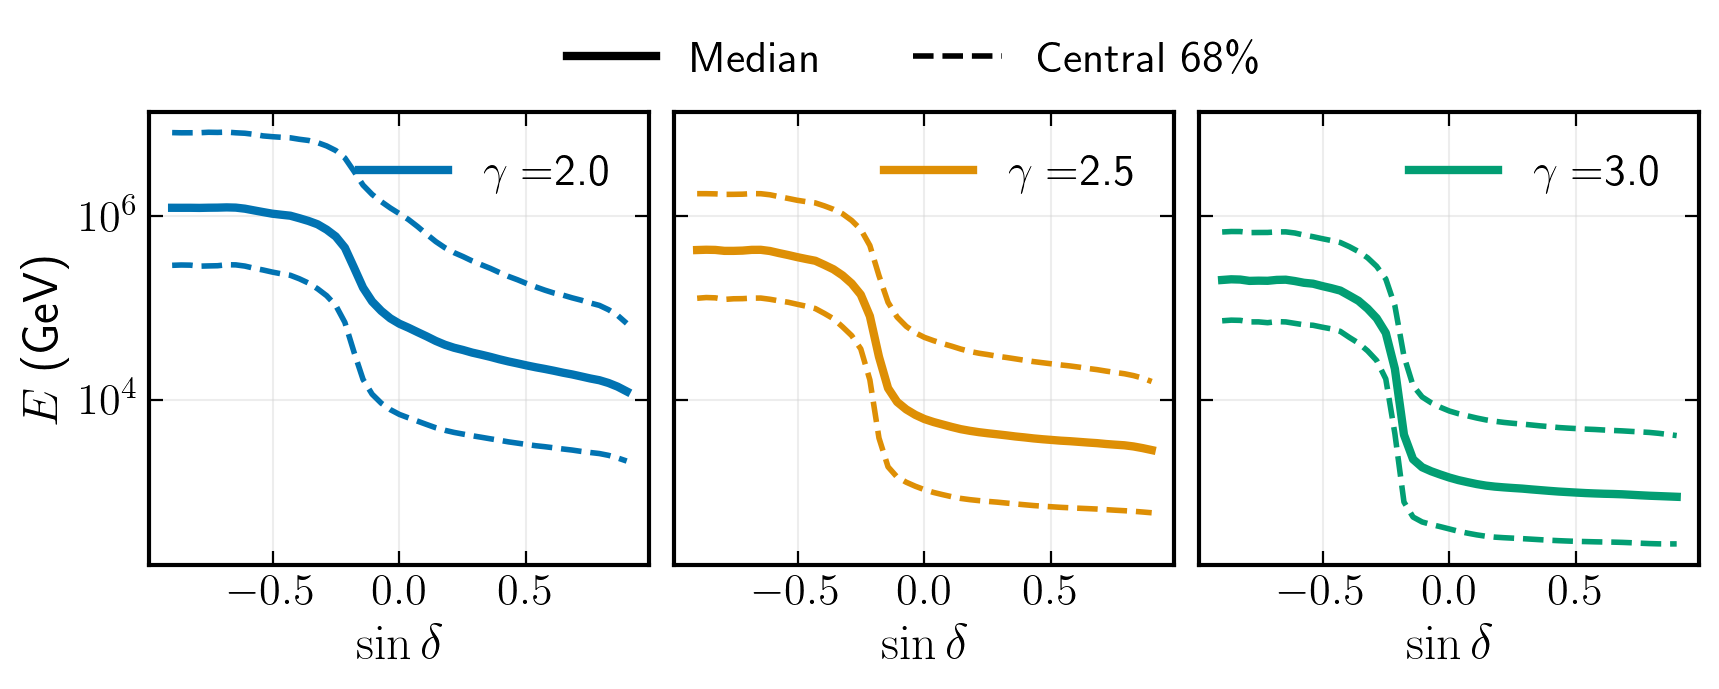
\includegraphics[width=0.95\textwidth]{figures/gfu_central_energies_effective_area.png}
    \caption{Central 68\% energy range calculated with the effective area construction for the GFU sample as a function of declination, for a variety of spectral indices.}
    \label{fig:central_en_eff_area_gfu}
\end{figure}

This is equivalent to weighting a Monte Carlo sample of events by the assumed spectral shape and calculating the CDF of the true neutrino energies. Finding where this CDF is equal to $\frac{1\mp\alpha}{2}$ will yield the relevant threshold energies. Figure~\ref{fig:central_en_eff_area_gfu} displays these energy ranges with $\alpha=0.68$ using the GFU sample (\texttt{GFUv002p05}). The central energy ranges calculated with a different event selection would of course differ, but they should be similar for other high-statistics, background dominated, track-based selections. This method has the advantage of a small computation time. 

\textbf{Sensitivity Construction.} The sensitivity construction answers a similar, albeit slightly different, question when compared to the effective area construction. This construction answers the question ``for a given assumed spectral hypothesis, which energies contribute most to the sensitivity of the analysis?'' To calculate this range, first find the sensitivity flux using the standard procedure (see Eq.~\ref{eq:sens}), call this value $\phi_{\mathrm{sens}}$. Then, repeat the calculation, but when initializing the analysis introduce a threshold, $E_{\mathrm{cut}}$ and exclude all signal events where $E_{\nu, \mathrm{true}} < E_{\mathrm{cut}}$. Float the threshold energy until the flux needed for sensitivity is $\phi_{\mathrm{sens}} \big/ \big( \frac{1+\alpha}{2} \big)$. Next, repeat this procedure, but this time place a cut on the highest energy events, excluding events with $E_{\nu, \mathrm{true}} > E_{\mathrm{cut}}$. Figure~\ref{fig:central_en_sensitivity_gfu} shows how this was calculated for a sample single point source analysis. This method is significantly more computationally intensive, as it requires the analyzer to recalculate the sensitivity of the analysis for a multitude of allowable $E_{\mathrm{cut}}$ values. 

\begin{figure}
    \centering
    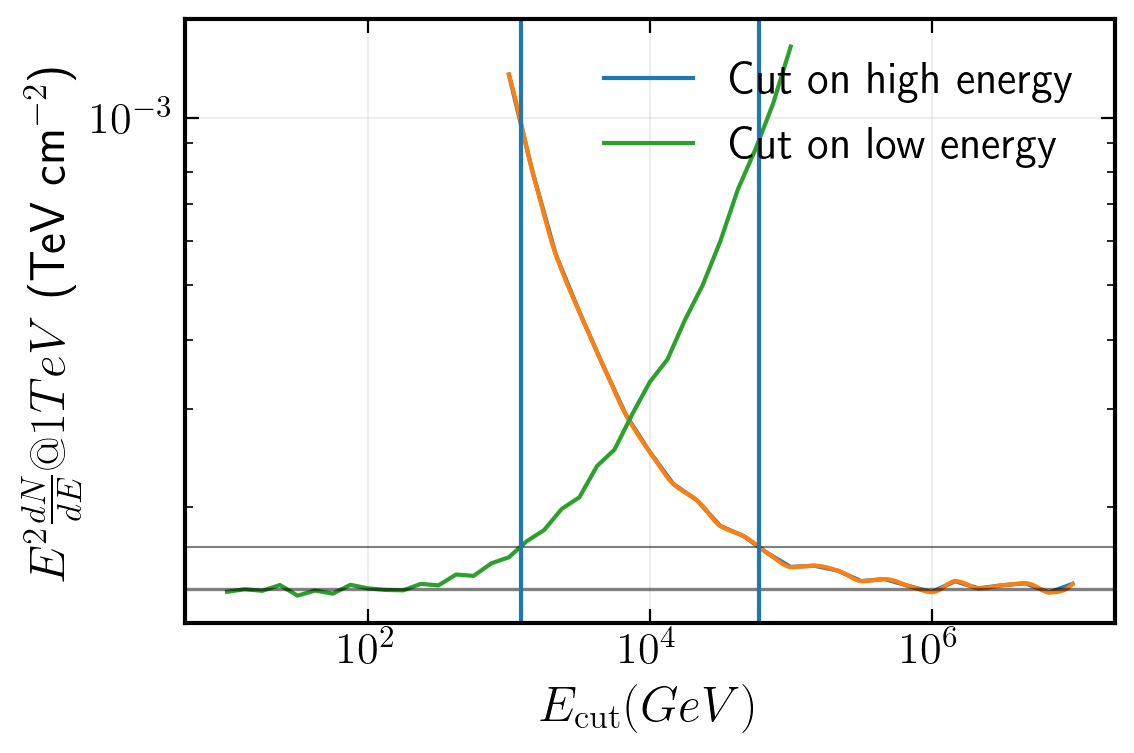
\includegraphics[width=0.5\textwidth]{figures/sensitivity_en_range_gfu.png}
    \caption{Sensitivity for a single source at $\delta=0^{\circ}$, with an analysis time window of $10^5$ s and an injected spectral index of $\gamma=2.5$. The lower and higher horizontal lines show $\phi_{\mathrm{sens}}$ and  $\frac{2\phi_{\mathrm{sens}}}{1+\alpha}$, respectively, with $\alpha=0.68$. The threshold energies are shown with vertical lines.}
    \label{fig:central_en_sensitivity_gfu}
\end{figure}

These methods are similar in motivation, but for large background analyses the energy ranges which we calculate can differ. However, for short timescales, the methods are equivalent. This is because at short timescales, our likelihood analyses function as counting experiments, and any signal event will yield a significant result. In this regime, the only thing that will affect the sensitivity is the detector response, meaning that the sensitivity will scale inversely and linearly with the effective area. Finding where the sensitivity degrades by a fraction of $\frac{1-\alpha}{2}$ is then the same as asking where the effective area is reduced by the same factor.

\begin{figure}
    \centering
    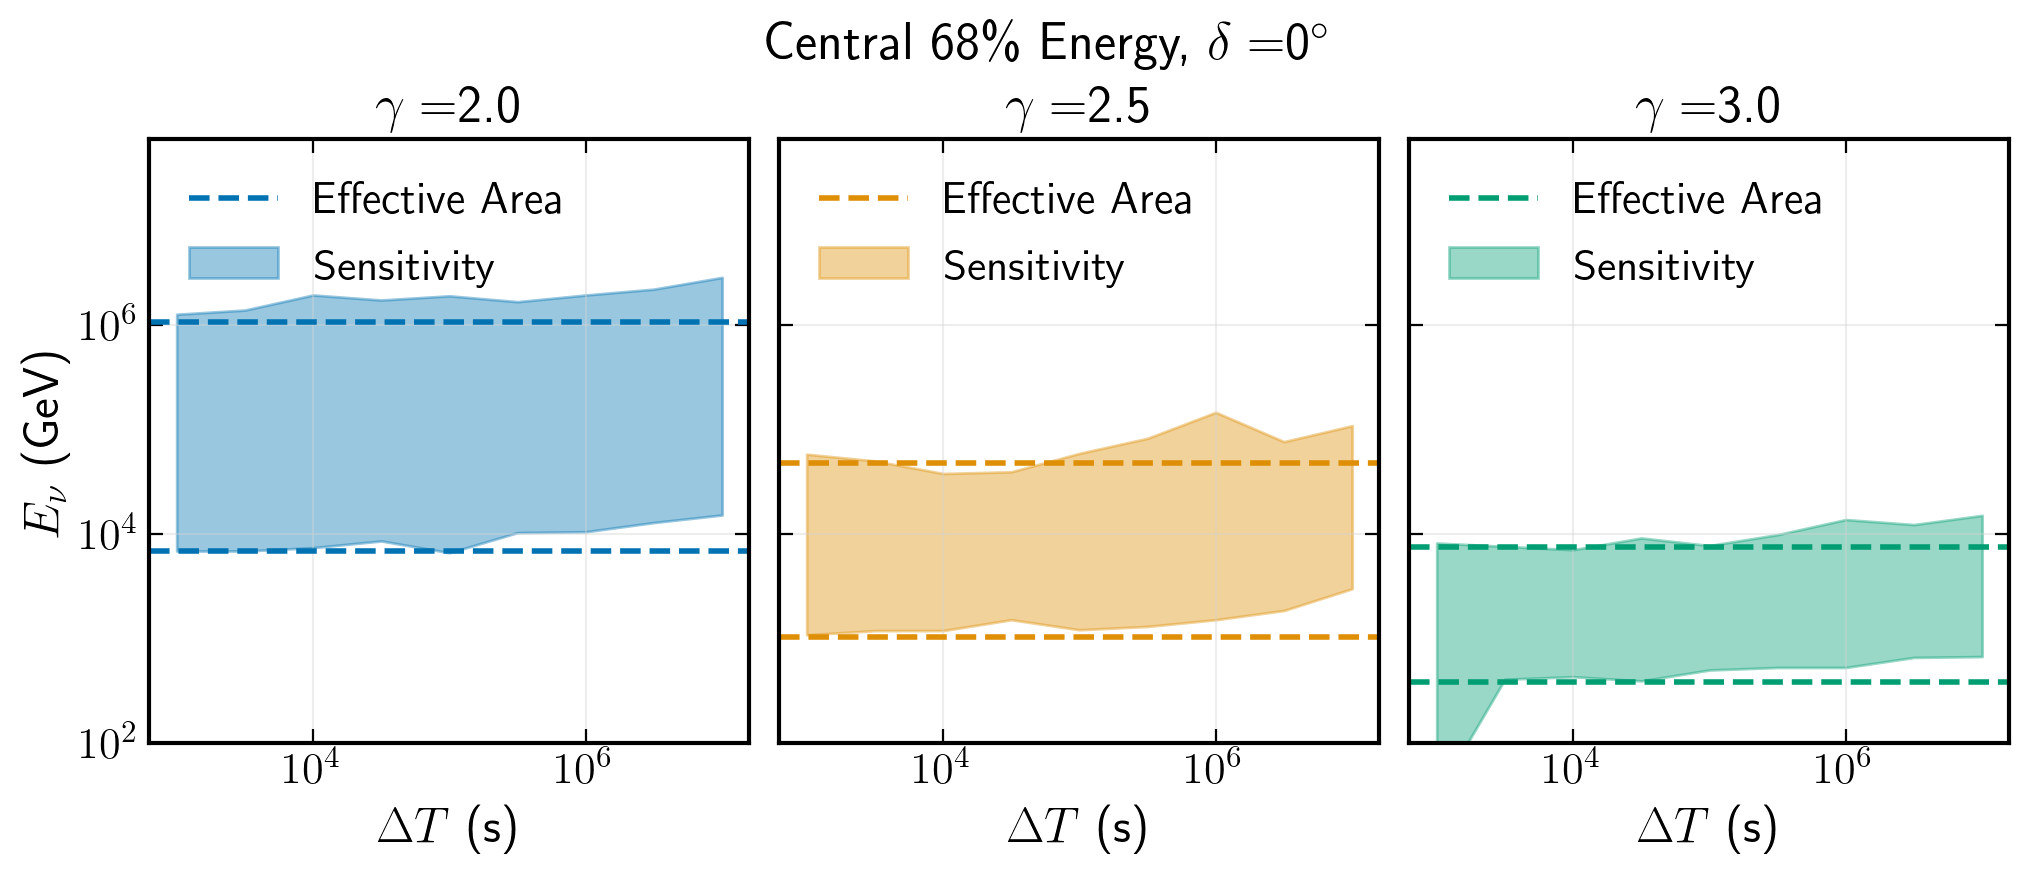
\includegraphics[width=0.98\textwidth]{figures/central_en_comparison_gfu.png}
    \caption{Central energy ranges under the ``effective area'' construction (dashed) and the ``sensitivity'' construction (shaded) for three different spectral indices. For short timescale analyses, the methods are equivalent, but diverge for larger time windows where the sensitivity construction will shift towards higher energy events.}
    \label{fig:energy_range_comparison}
\end{figure}

Figure~\ref{fig:energy_range_comparison} shows this comparison explicitly, for a source at the horizon. This Figure highlights that for small background (short timescale) analyses, the two constructions are equivalent. However, for larger time windows, the extra per-event information becomes important, and the energy range which contributes to the sensitivity shifts towards higher energies, where events on average are better reconstructed and are easier to distinguish from background. For this reason, we recommend the analyzer use the ``effective area'' construction for short timescale (ie low-background) analyses, to reduce the computational requirements. For longer timescales, it is up to the analyzer to decide which question is more prudent for their analysis. It is worth noting that all of the examples in the Figures above set $\alpha=0.68$ in order to minimize the statistics needed in calculating various sensitivities, though all of the same logic holds for the more common convention of $\alpha=0.90$. 

\subsection{Pivot Energies}
\label{subsec:pivot}
It is sometimes the case that analyzers wish to calculate their sensitivity for a variety of spectral indices for simple power laws. In this case, it becomes cumbersome to quote (or plot) all of these fluxes in a compact way. One way around this is to plot the sensitivity flux at the pivot energy $E_0$ as a function of spectral index, $\gamma$. For an example of this in a recent paper, see Figure 2 of \cite{ICECUBE:2021edr}. However, to accomplish this, one must choose a specific reference point to quote all fluxes at, and as discussed above, the central energy range of an analysis is dependent upon the assumed spectral shape being tested. 

These visualizations, while completely correct, have induced some confusion, as the choice of pivot energy is arbitrary but not without impact. At first glance, choosing a higher pivot energy, $E_0$, when defining your flux might make it appear as if the analysis is more sensitive to softer spectral indices than harder spectral indices. This is shown in Figure~\ref{fig:pivot_energies}, with the sensitivity to a point source for three different spectral indices shown on the left. These spectra are also parameterized on the right for three different choices of pivot energies. While all three lines on the right parameterize the same set of fluxes, note that in the figure some of the choices of pivot energy are within the central energy range for certain spectral shapes and not for others. While there is not a single ``best pivot energy'' to quote, it is probably best to choose a pivot energy that is within as many central energy ranges as possible for the different spectral indices being tested (note how this is the case in \cite{ICECUBE:2021edr}, as the pivot energy of 10 TeV is roughly within all of the central energy ranges shown in the left hand side of Figure 3).

\begin{figure}
    \centering
    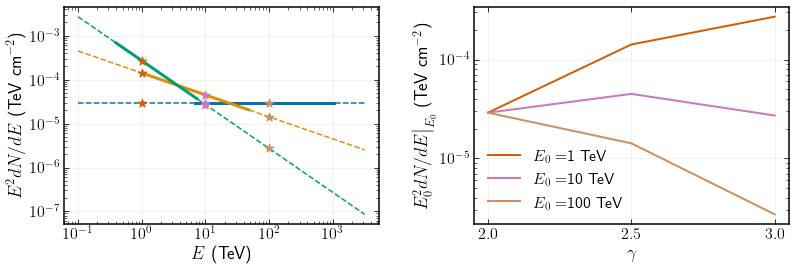
\includegraphics[width=0.90\textwidth]{figures/pivot_energies.png}
    \caption{Sensitivity to a point source at the horizon with three different spectral assumptions (left). Solid lines denote where we expect the central 68\% of signal events for each spectral assumption, ie the effective area construction of central energies. The plot on the right shows what the sensitivity at the pivot energy as a function of spectral index, and the stars in the left hand plot share the same color scheme, to highlight where in each spectrum we are calculating the flux.}
    \label{fig:pivot_energies}
\end{figure}

\section{Time-integrated fluxes and ``Fluence''}
Arguably just as important as the energy range is the magnitude of flux at which an analysis is most sensitive. For analyses that test non-steady temporal hypothesis (eg. ``transient'' analyses or ``flare'' analyses), there is the added confusion of describing this flux succinctly even though it changes as a function of time. To get around this problem, we often describe fluxes in terms of time-integrated quantities, i.e. in terms of a ``fluence''. There are a few different conventions -- all of which correspond to slightly different physical quantities -- which we outline below.
\begin{enumerate}
    \item Time-integrated differential energy flux, $\mathcal{F}$ (``particle fluence''):
    \begin{equation}
        \mathcal{F}(E) = \int \frac{dN}{dEdAdT} dT
    \end{equation}
    \item ``Energy fluence,'' $\mathbb{F}(E_a, E_b)$:
    \begin{equation}
        \mathbb{F}(E_a, E_b) = \int\int_{E_a}^{E_b} E \frac{dN}{dEdAdT} dEdT
    \end{equation}
\end{enumerate}

Physically, these different fluences refer to two distinct quantities, as indicated by their names. The ``particle fluence,'' $\mathcal{F}(E)$, quantifies the \textit{number of particles of a certain energy that pass through an area in a given time}. The ``energy fluence,'' $\mathbb{F}(E_a, E_b)$, is the \textit{amount of energy in a flux per unit area in a given time over a specific energy interval}.

When quoting sensitivities, we often do this in terms of the particle fluence, $\mathcal{F}(E)$, scaled by a factor of energy-squared, $E^2\mathcal{F}(E)$ (in much of our internal software, such as \texttt{csky}, this quantity is called $E^2dN/dE$). Scaling a flux by $E^2$ has a variety of benefits -- it serves as a proxy for the energy content in a flux, when showing the flux over many orders of magnitudes subtle changes in slope become more apparent, and for the special case of the prototypical $E^{-2}$ this quantity is independent of energy. To make matters more confusing, $E^2\mathcal{F}(E)$ is also sometimes referred to as the ``neutrino spectral fluence.''

Both of these quantities, $E^2\mathcal{F}(E)$, and $\mathbb{F}(E_a, E_b)$ are extremely informative. For example, $E^2\mathcal{F}(E) = \Delta T \times E \times dN / d\log E$, is analogous to the time-integrated spectral energy density, $\nu F(\nu)$ used ubiquitously in multi-wavelength astronomy, which shows the energy content per logarithmic interval of energy and thus serves as an intermediary for the physics of an astrophysical source \cite{Gaisser:2016uoy}.

However, these quantities are distinct, and although the difference is subtle, the energy scaling of particle fluence results in a confusion between these two quantities, as the units of these quantities are equal:
\begin{equation}
    \big[E^2\mathcal{F}(E)\big] = \big[\mathbb{F}(E_a, E_b)\big] = \mathrm{GeV}\;\mathrm{cm}^{-2}\;,
\end{equation}
and also because in some papers we have a tendency to just quote the ``fluence'' (or sometimes ``neutrino fluence'') needed for sensitivity instead of clarifying if this ``fluence'' is an energy fluence or energy-squared times particle fluence (see the following section for a list of where this has recently appeared in the literature). This leads to confusion when we just quote ``a fluence of $x$ GeV cm$^{-2}$,'' which at face value seems like an energy fluence as it is not clear over what energy range this is applicable. However, we are usually discussing a particle fluence at a particular energy, which is not clear because we do not specify that we have scaled a particle fluence by $E^2$ to have these units, or because for an $E^{-2}$ this is independent of energy and so a specific pivot energy need not be specified.

Although we normally discuss particle fluences for sensitivities, we still often want to calculate the energy in a flux, for which we need to specify an energy interval. For calculating the energy interval, we often use the methods outlined in Section~\ref{sec:energy_range}.

\subsection{Example: Power-laws}
Suppose we have an astrophysical source which emits neutrinos according to a power-law spectrum, 
\begin{equation}
    \frac{dN}{dEdAdT}= \phi_0 \Big(\frac{E}{E_0}\Big)^{-\gamma} \; ,
\end{equation}
and we collect data on this source for an observation period of $\Delta T$. The energy-scaled time-integrated differential energy flux and the energy fluence are calculated as 
\begin{equation*}
\begin{aligned}[c]
    E^2\mathcal{F}(E) &= E^2\int \frac{dN}{dEdAdT} dT \\
    &= E^2 \Delta T \phi_0 \Big(\frac{E}{E_0}\Big)^{-\gamma} \\
    &= \phi_0 E_0^{\gamma} E^{2-\gamma}\Delta T
\end{aligned}
\qquad\&\qquad
\begin{aligned}[c]
    \mathbb{F}(E_a, E_b) &= \int dT \int_{E_a}^{E_b} E \frac{dN}{dEdAdT} dE \\ 
    &= \Delta T \int_{E_a}^{E_b} E \phi_0 \Big(\frac{E}{E_0}\Big)^{-\gamma} dE \\
    &= \phi_0 \Delta T E_0^{\gamma} \times \begin{cases}
            \ddfrac{E^{2-\gamma}}{2-\gamma}\Big|_{E_a}^{E_b} &\gamma\neq 2 \\ \log\big(\ddfrac{E_b}{E_a}\big) & \gamma = 2
        \end{cases}
\end{aligned}
\end{equation*}

In the case of $\gamma = 2$, we have 
\begin{equation}
    \frac{\mathbb{F}(E_a, E_b)}{E^2\mathcal{F}(E)} = \log\big(\ddfrac{E_b}{E_a}\big) \; ,
\end{equation}
so in the case of an $E^{-2}$, where the energy output per decade in energy is a constant, then we can interpret $E^2\mathcal{F}(E)$ as the energy fluence per logarithmic energy interval.

For all other spectral indices, we have
\begin{equation}
    \frac{\mathbb{F}(E_a, E_b)}{E^2\mathcal{F}(E)} = 
    \frac{1}{2-\gamma}\frac{E_b^{2-\gamma} - E_a^{2-\gamma}}{E^{2-\gamma}} \; ,
\end{equation}
and it is clear that we are not as able to draw immediate parallels between these two physical quantities.

It is also worth noting that in order to convert a flux to the amount of energy that an astrophysical source emits (or its luminosity for constant fluxes), one must properly take into account cosmic expansion and how this affects (1) the duration of a transient and (2) the energy of the particles emitted. For this entire discussion, we are assuming all times are in the observer frame. For more discussion on the differences between fluxes and fluences and between energy and particle fluxes, and specifically how they behave differently due to cosmic expansion, I would strongly recommend reading Appendix B of Nora Linn Strojohann's thesis \cite{norathesis}.

Moving forward, we would like to advocate that all fluxes are which are quoted are at some point defined explicitly in terms of their differential notation, as we did when introducing the difference between particle and energy fluence. We believe that ``energy-scaled time-integrated differential energy flux $E^2dN/dE\times \Delta T $'' is the most transparent quantity to quote as it does not rely on an energy interval whose determination is itself not fixed. Though it is not incorrect to name this quantity a sort of ``fluence,'' we would advocate not using such wording because of the confusions that were outlined in this Section, though ultimately this is up to the discretion of the analyzer / author. If the term ``fluence'' is used, it should always be specified whether this integrated over energy or a function of energy.

\subsection{A brief literature review}
Keeping these conventions straight is not always easy, and it is not only IceCube that has used the word ``fluence'' vaguely without clarifying which physical quantity is being shown. Below is a list of papers that use the term ``fluence,'' organized into those that mean it as ``particle fluence'' and those that mean ``energy fluence.'' It is only a subset of these papers that explicitly define these quantities. Links in \textcolor{magenta}{magenta} are IceCube papers, and links in \textcolor{PineGreen}{green} are external. 

\begin{table}[h]
    \centering
    \begin{tabular}{|p{0.4\linewidth}|p{0.4\linewidth}|}
          \hline Particle Fluence & Energy Fluence \\ \hline 
    \arxiv[PineGreen]{1906.07209}\tablefootnote{Error in Eq. 17, saying particle fluence has units energy per unit area} & \arxiv[magenta]{1611.03062} \\
    \arxiv[magenta]{1712.06277} & \arxiv[PineGreen]{1902.09462} \\
    \arxiv[PineGreen]{1812.11673} & \arxiv[magenta]{2012.01079}  \\
   \arxiv[PineGreen]{2102.02223} & \arxiv[PineGreen]{2103.15526} \\ 
   \arxiv[PineGreen]{1906.07209} & \arxiv[PineGreen]{1902.09462} \\ 
   \arxiv[PineGreen]{1812.11673} & \arxiv[magenta]{1503.00598} \\ 
   \arxiv[magenta]{2004.02910} & \\ 
   \arxiv[PineGreen]{2103.16577} & \\
   \arxiv[magenta]{2101.00610} & \\
   \arxiv[magenta]{2011.05096} & \\
   \arxiv[PineGreen]{2010.02869} & \\
   \hline
    \end{tabular}
    \label{tab:my_label}
\end{table}

Additionally, there are some papers where it is unclear what quantity ``fluence'' refers to (eg. \arxiv[PineGreen]{2011.02452}), or that use ``fluence'' to mean both energy-squared times particle fluence as well as energy fluence, depending on a context that isn't always clear (eg \arxiv[PineGreen]{1611.03062}, \arxiv[PineGreen]{2008.12318}, \arxiv[PineGreen]{2007.15742}). The latter is most frequently when using ``fluence'' to describe an energy integrated quantity when comparing to multi-wavelength bands, but $E^2$ times particle fluence for neutrinos. This list is by no means exhaustive (it was only the first few years reverse chronologically from an arXiv search for the words ``IceCube'' and ``fluence'').

\section{Differential Sensitivity}
One method to convey the response of an analysis as a function of energy is through a \textit{differential sensitivity}. We will keep this section brief, as all of the technical material covered in this section is covered in depth in \cite{Rene:differential}. However, we want to discuss a few of the current conventions in the working group below.

\begin{figure}
    \centering
    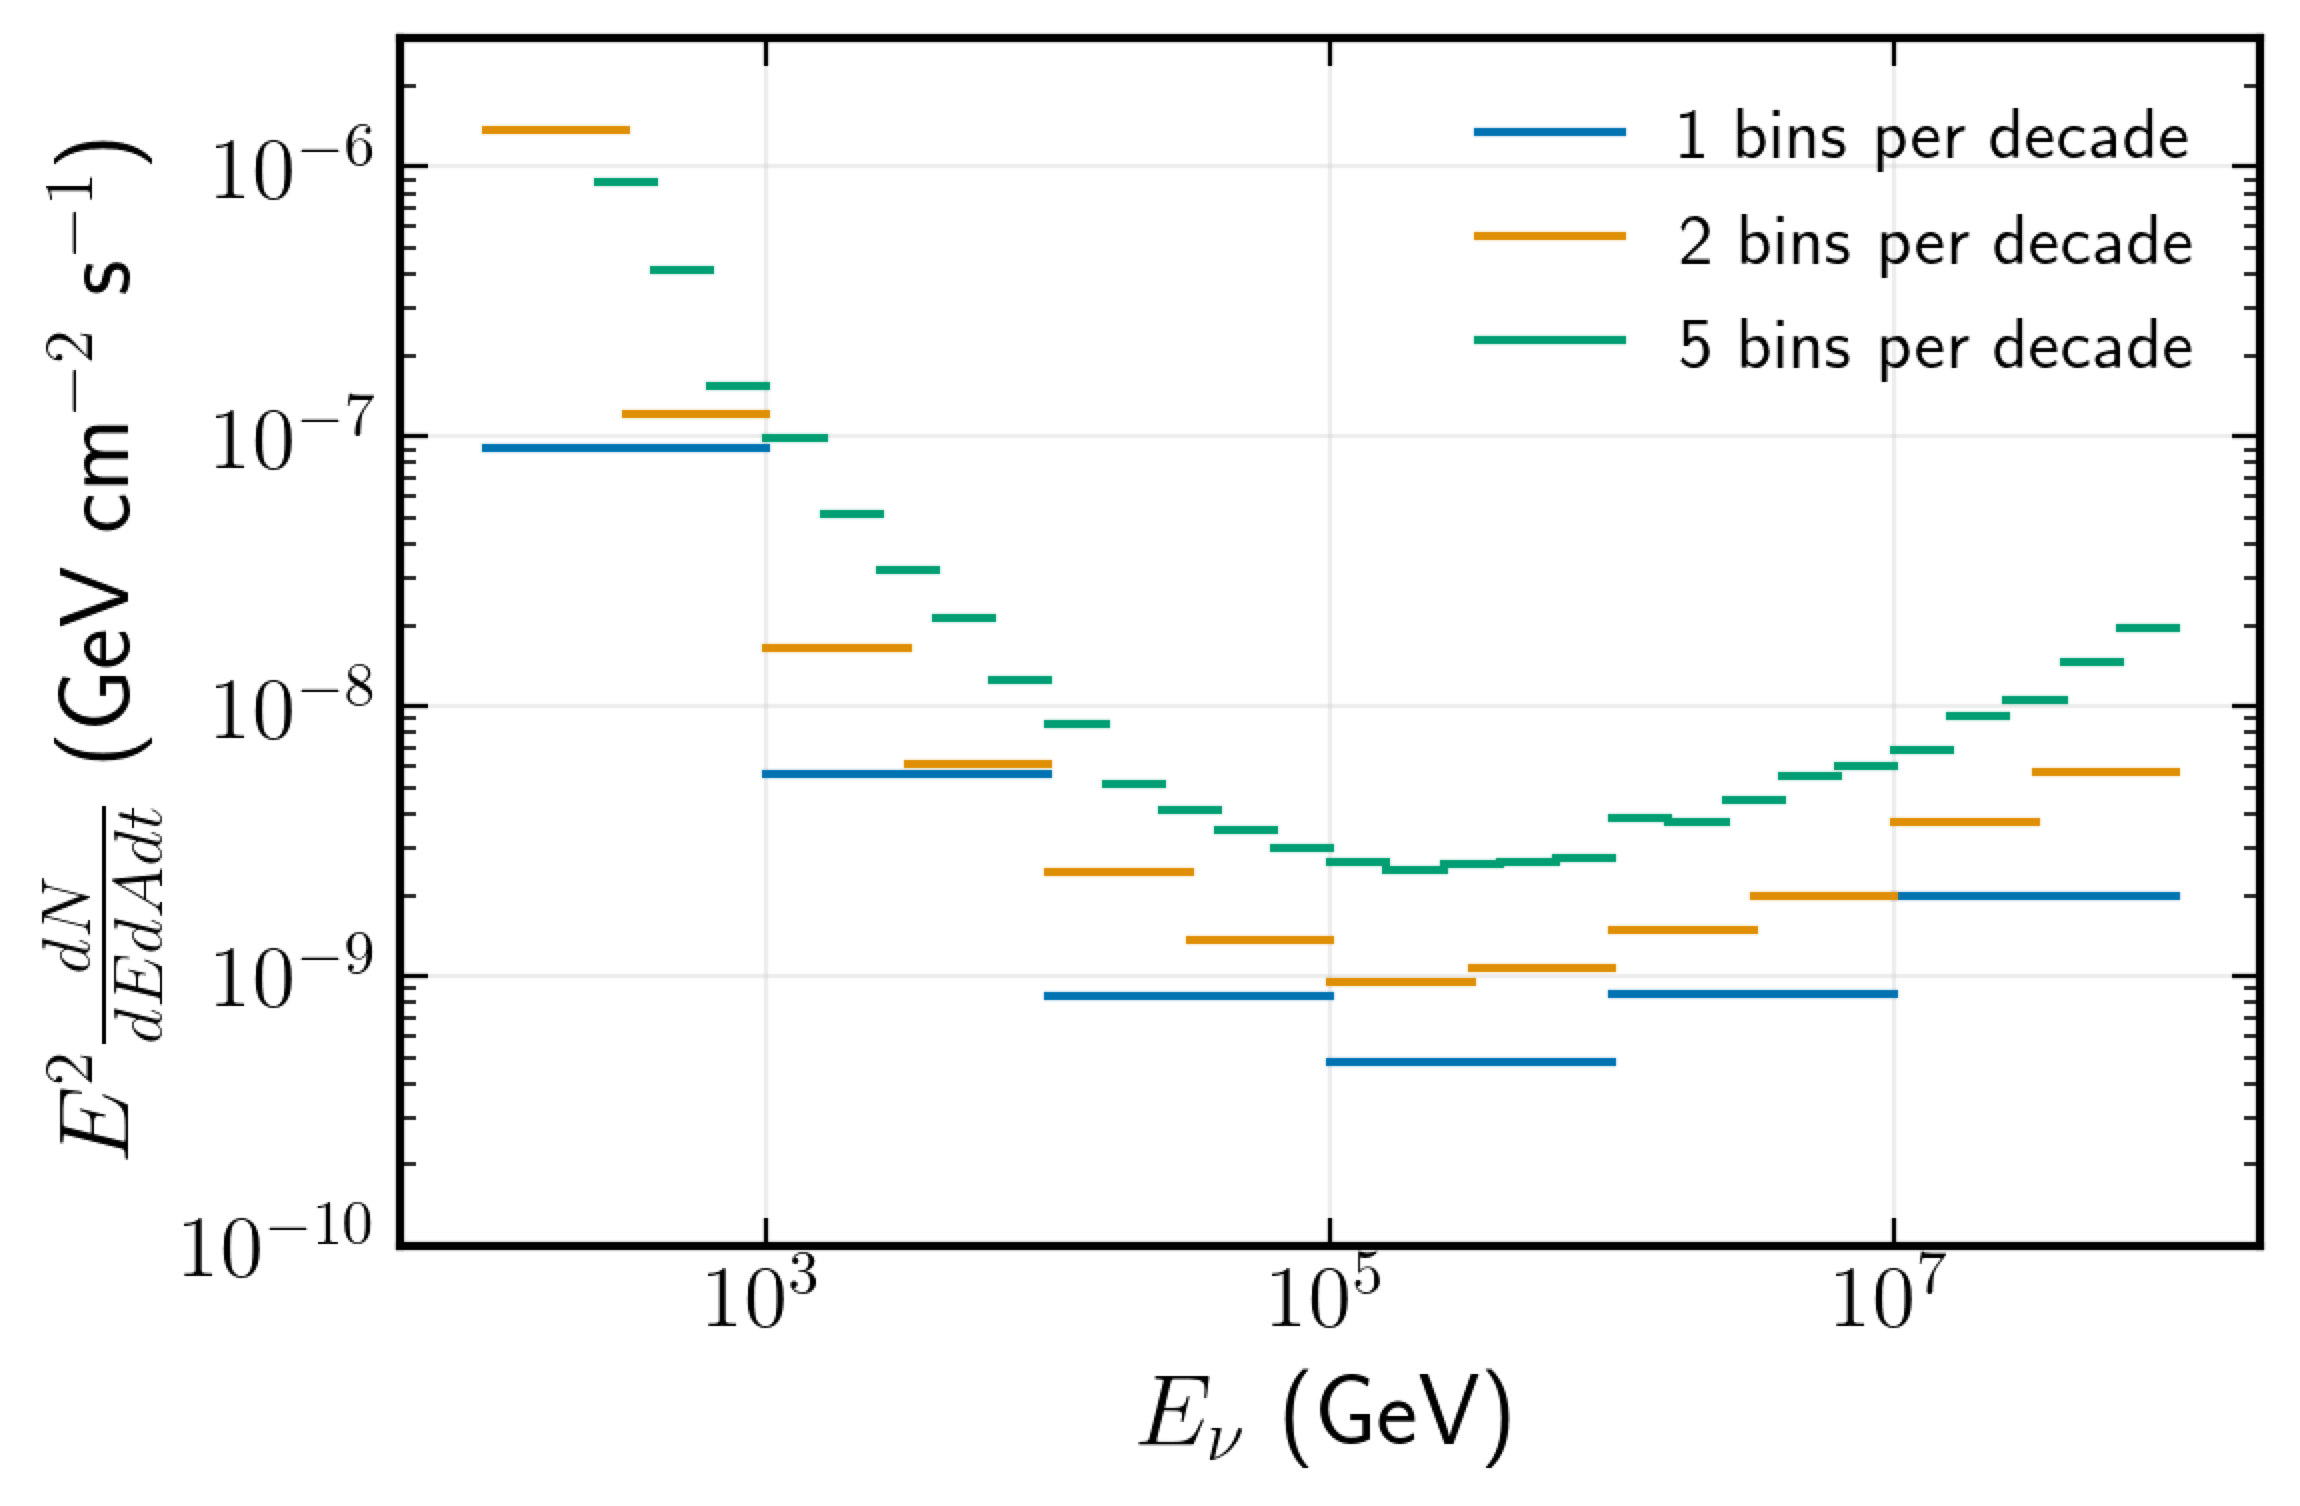
\includegraphics[width=0.49\textwidth]{figures/differential_sens_bin_width.png}
    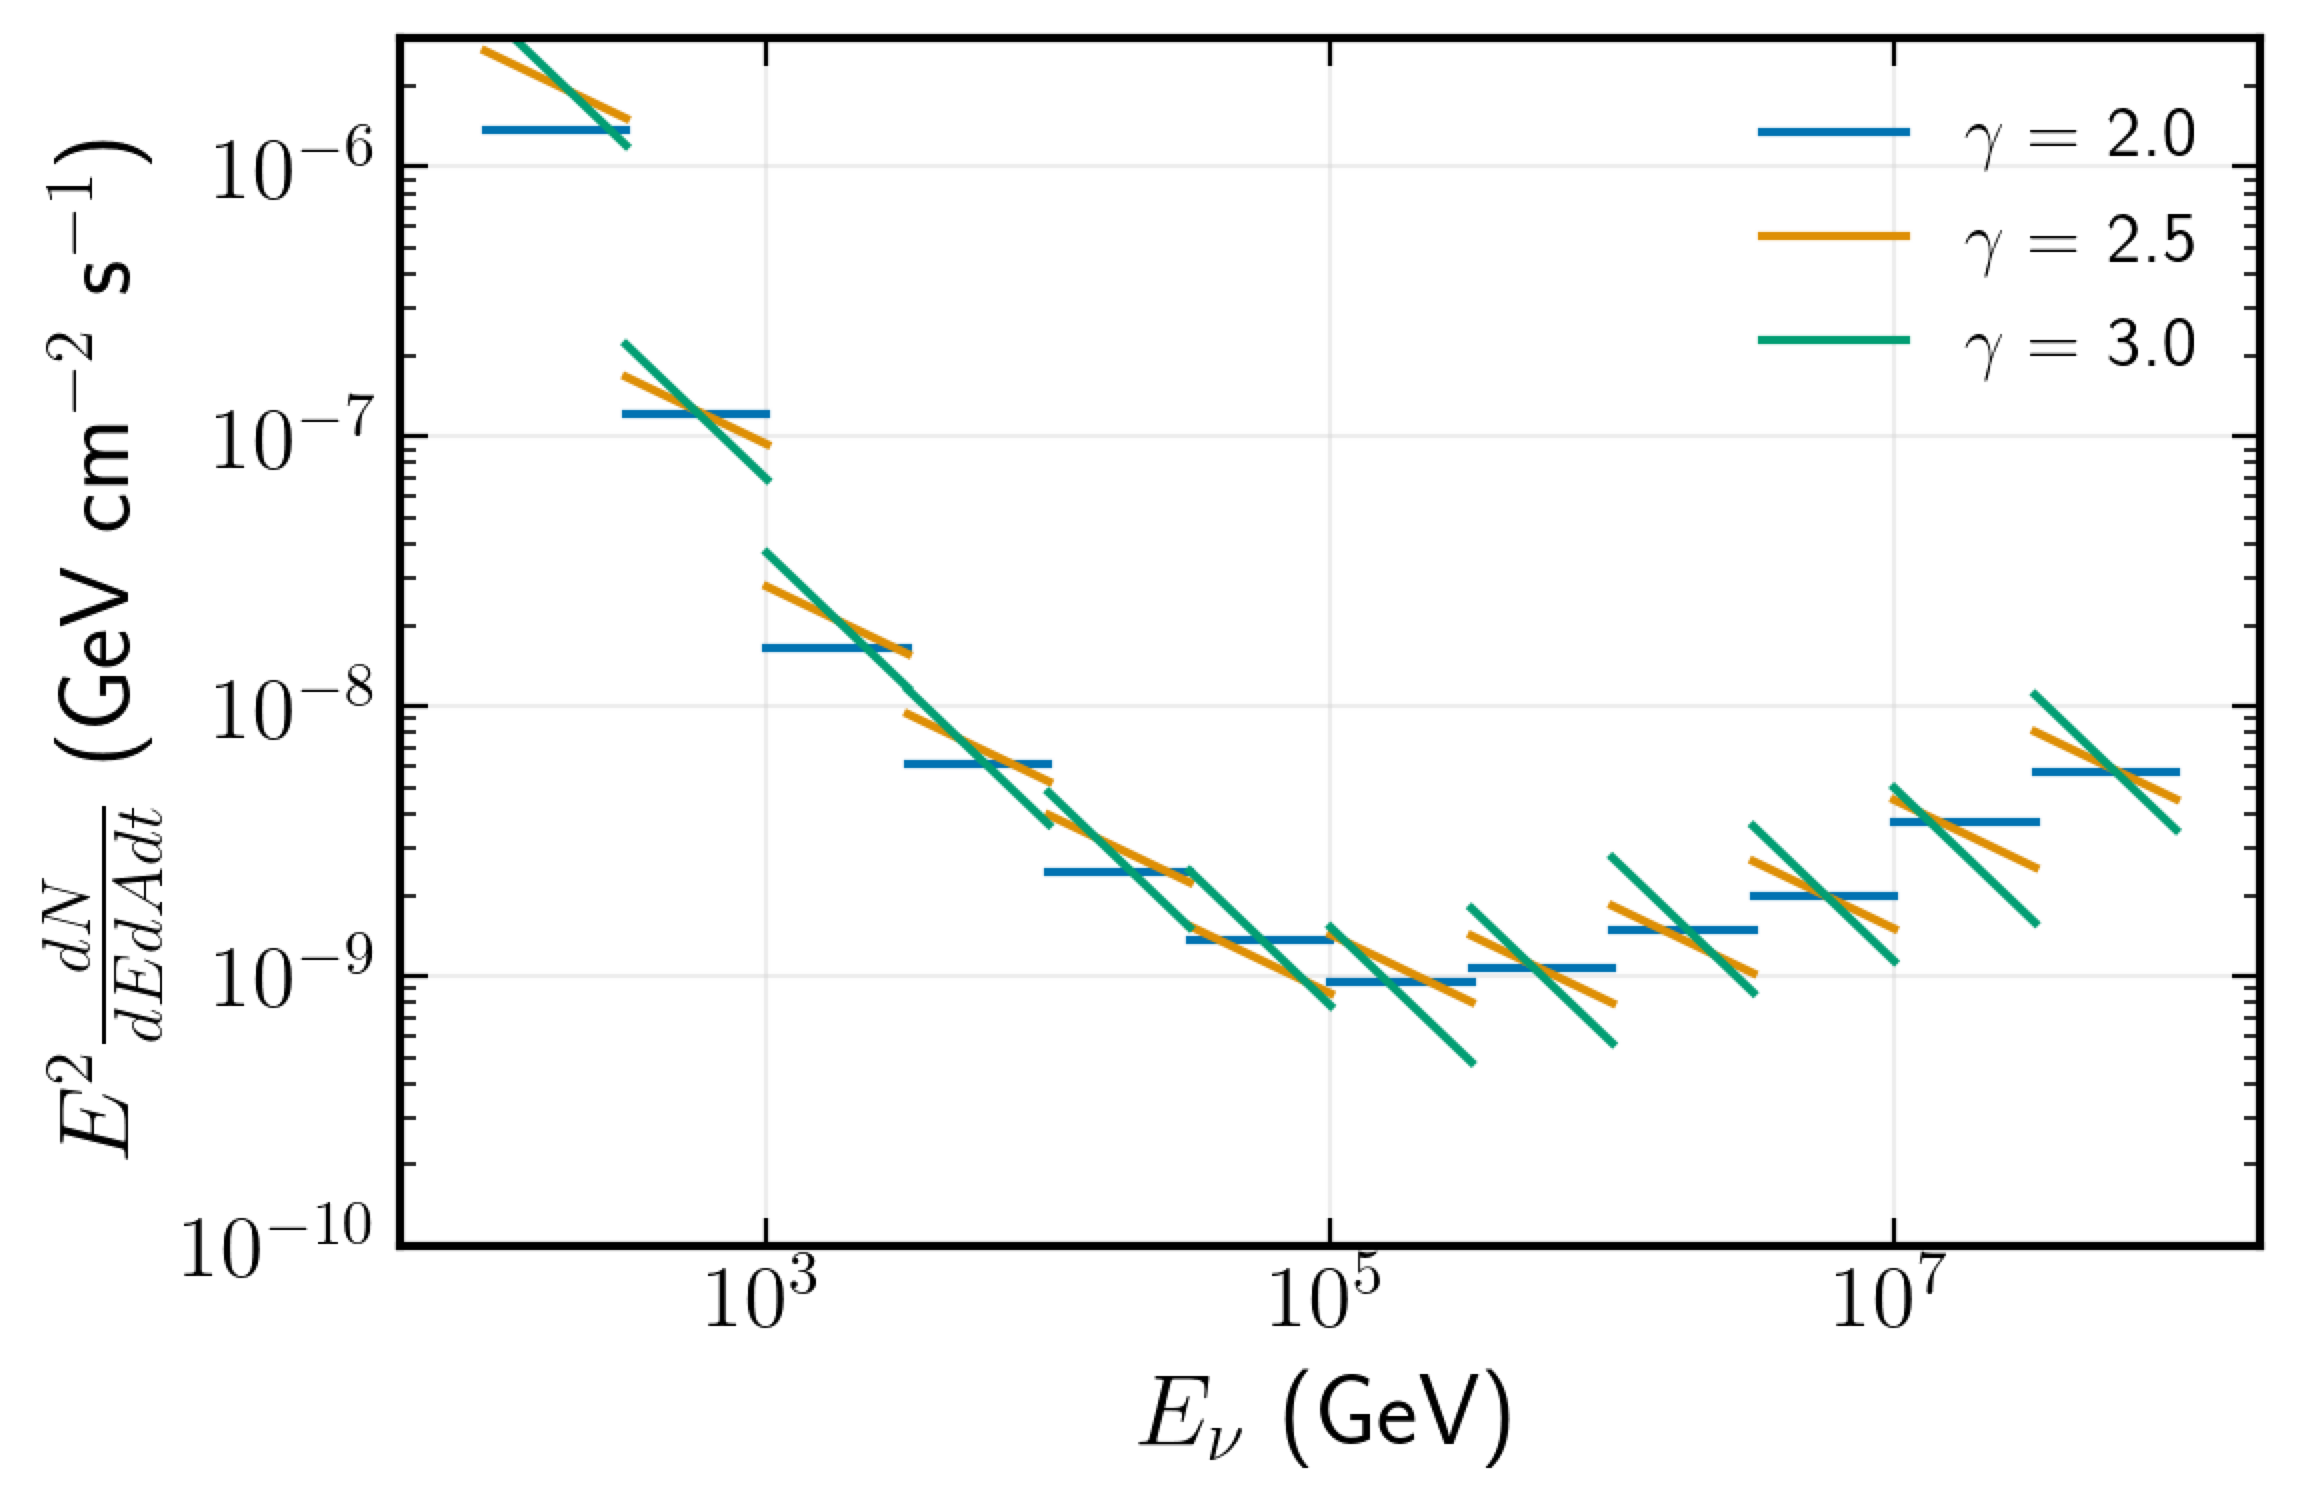
\includegraphics[width=0.49\textwidth]{figures/differential_injected_index.png}
    \caption{Differential sensitivity for a time-integrated point source analysis using \texttt{PSTracks\_v4} for a source at the horizon, $\delta=0^{\circ}$. The differential sensitivity is subject to a variety of convention choices such as the bin width (left) or the assumed spectral index (right) within each bin. While all of the curves reflect similar behaviors as a function of energy, the normalization of these fluxes is a function of the bin width and thus the convention choice can obfuscate which spectral models to which this analysis would be sensitive.}
    \label{fig:diff_sens_conventions}
\end{figure}

To construct a differential sensitivity, follow the same process as when calculating a normal sensitivity, but under the assumption that the flux model is valid only over a finite range $[E_{\mathrm{min}}, E_{\mathrm{max}}]$, and is 0 elsewhere. Then, to construct the full differential sensitivity, repeat this for a variety of energy intervals. The differential sensitivity, then, is not only a function of the assumed spectral shape within the energy interval, but also of the size of the energy interval. For example, assume a detector has 100\% detection efficiency across a range $[E_a, E_b]$ and has a differential sensitivity equal to $\phi_0$ for this energy interval. If we instead calculate the differential sensitivity for the energy ranges  $[E_a, \frac{E_a + E_b}{2}]$ and $[\frac{E_a + E_b}{2}, E_b]$, the differential sensitivity in each of these bins will be equal to $2\phi_0$. This effect is highlighted in Figure~\ref{fig:diff_sens_conventions}, where we show that the differential sensitivity is not only a function of the bin-width but also the assumed spectral index within each bin (it is also common in some fields to flatten steeper powers of energy by scaling the y-axis by a power besides $E^2$, such as when showing cosmic-ray fluxes).

This becomes especially confusing when trying to compare a differential sensitivity against a predicted energy-scaled particle fluence from a model, as has become commonplace in many of the WG's recent works. When doing this comparison, it is not enough to see if a model curve crosses over a binned differential sensitivity. In reality, the model would contribute to every energy interval, not just over the finite bins that have been chosen for visualization. As such, we are often underselling our analysis sensitivity, because we are sensitive to some models that do not cross over the individual differential sensitivity curves at all because there are contributions in many energy intervals. 

\begin{figure}
    \centering
    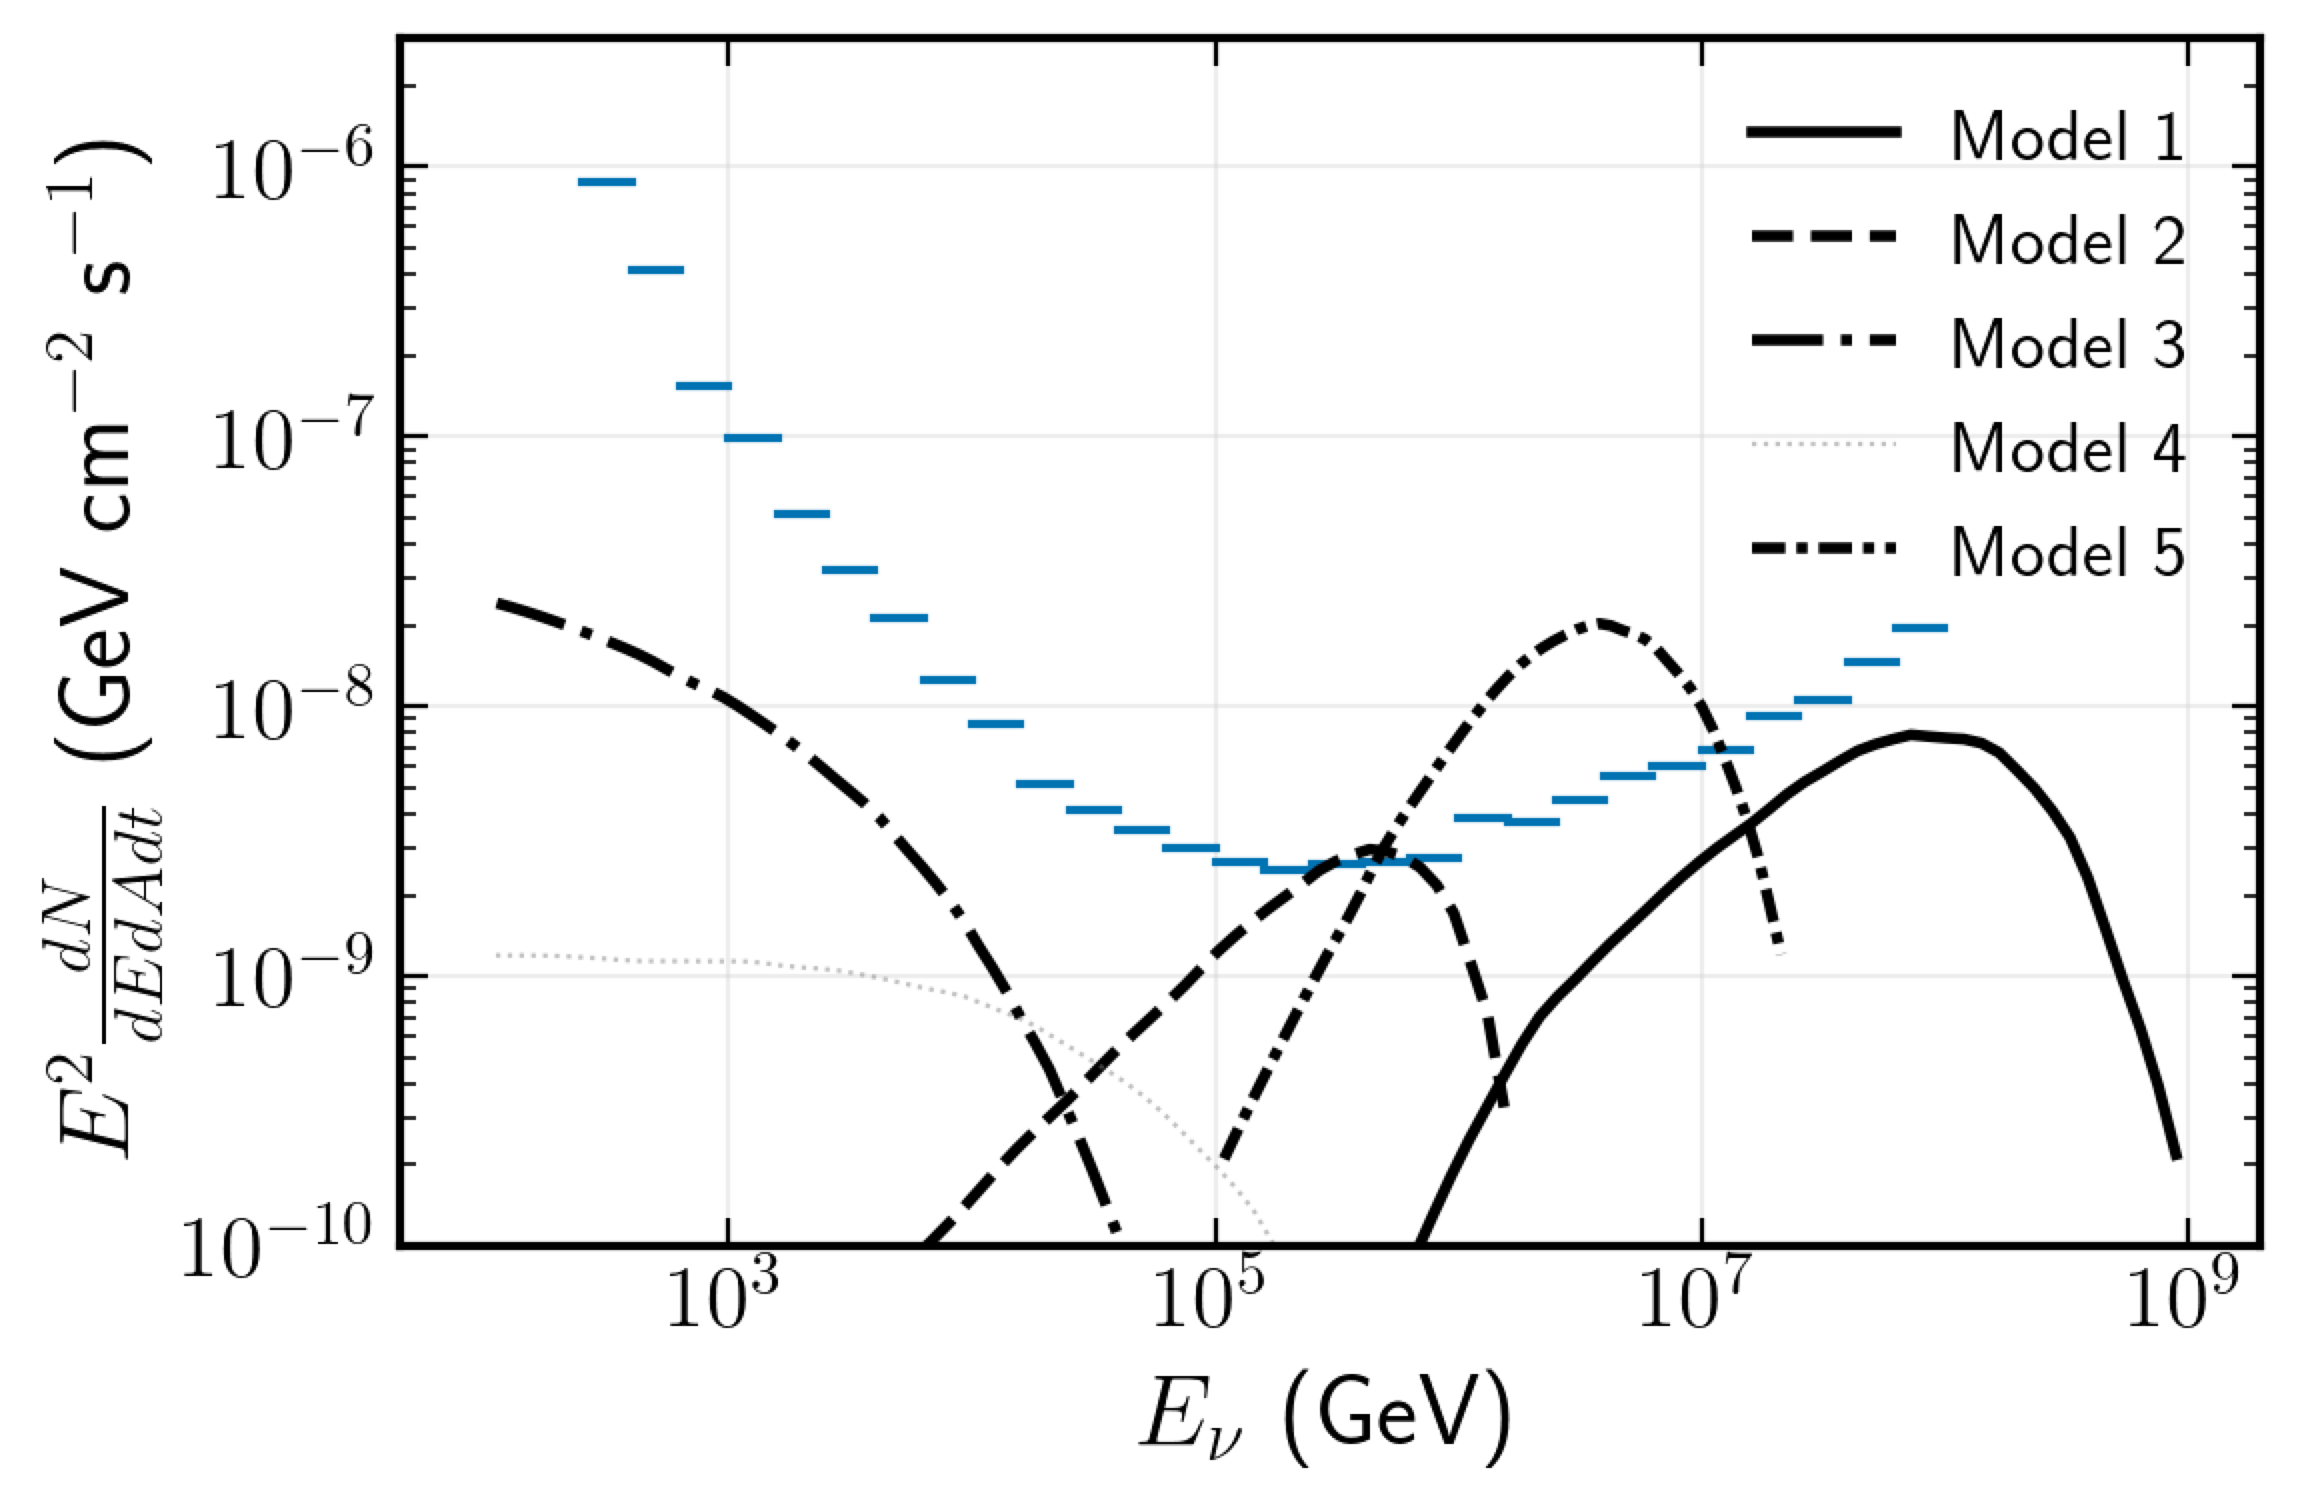
\includegraphics[width=0.48\textwidth]{figures/differential_highlighted_sensitive.png}
    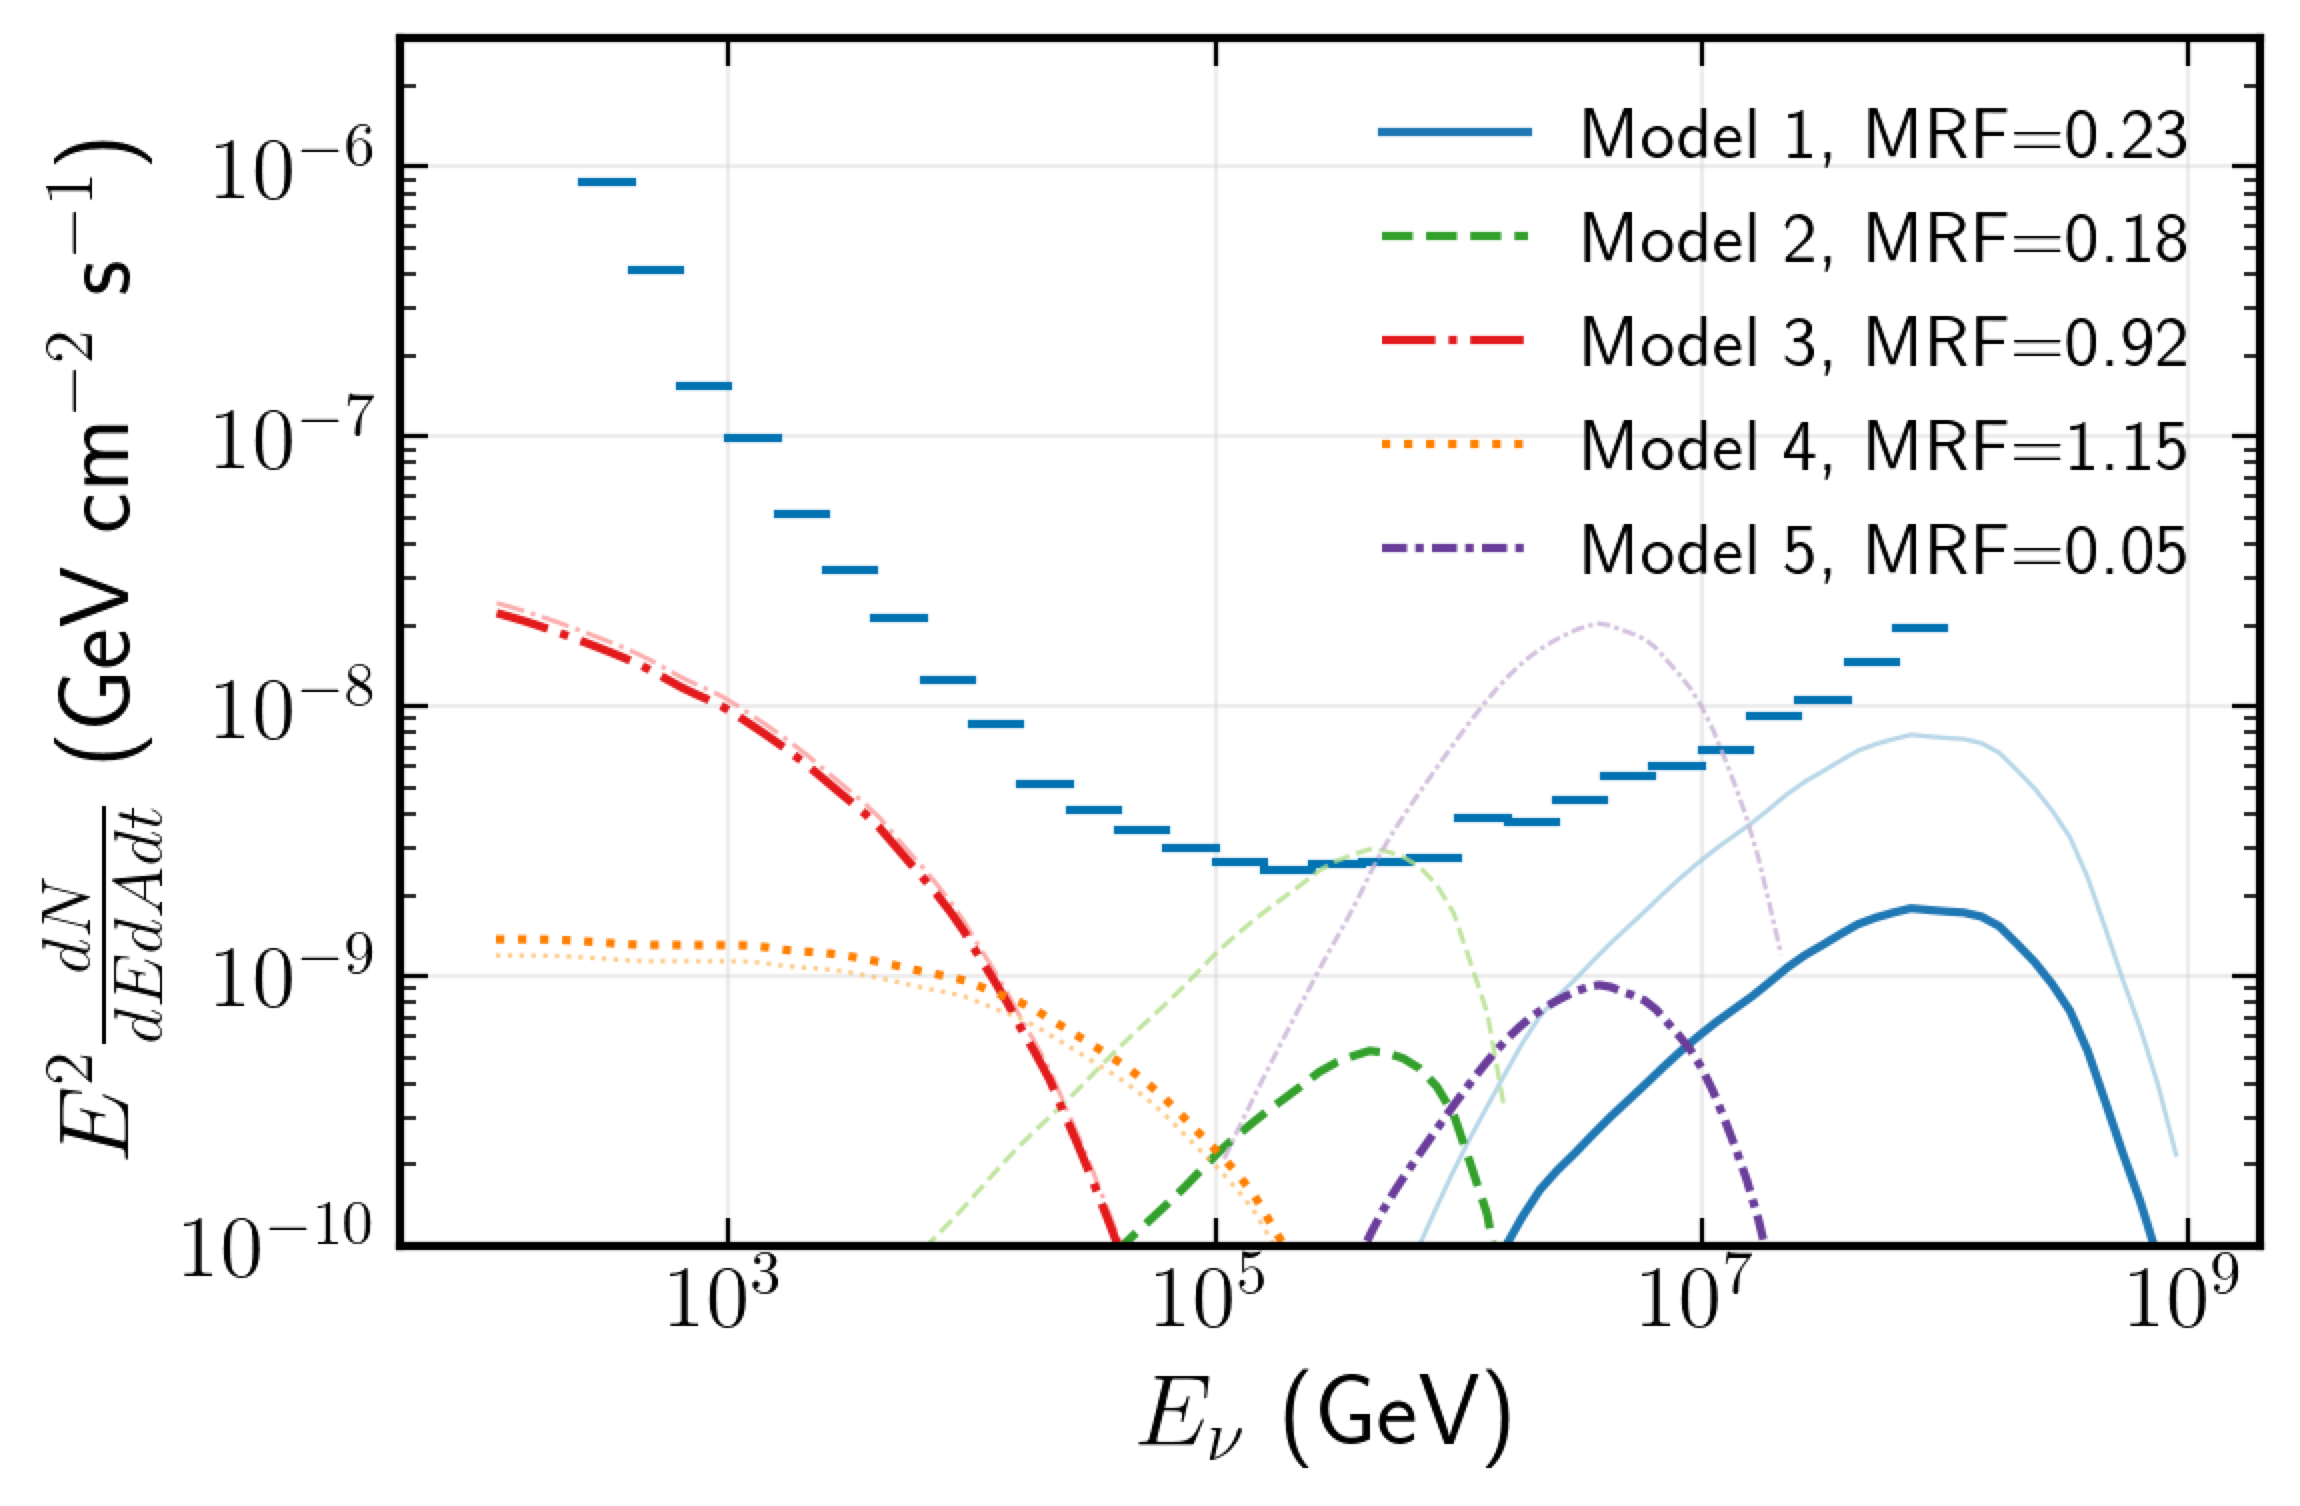
\includegraphics[width=0.48\textwidth]{figures/differential_with_mrf.png}
    \caption{Differential sensitivity overlaid with various toy model predictions. In the left, those models to which the analysis is sensitive are shown in black while the model which is below our detection threshold is shown in gray. Even though models 1 and 3 do not cross the differential sensitivity curve, the analysis is still sensitive to them. In the right, we show the same model predictions in lighter and narrower curves, and the heavier and darker colors show the spectral shapes scaled by their (expected) model rejection factors to show the threshold for sensitivity for these models.}
    \label{fig:diff_sens_mrf}
\end{figure}

This is shown in Figure~\ref{fig:diff_sens_mrf}, where we show an analysis differential sensitivity with 5 bins per decade for a source at $\delta=30^{\circ}$ using \texttt{PSTracks\_v4}. In the figure on the left, those models to which the analysis is sensitive are highlighted in black, and it is clear that even though some models never cross over individual line segments from the differential sensitivity, the contributions over multiple energy intervals add up to a signal to which the analysis is sensitive. 

We show one of the ways to avoid this confusion in the right of Figure~\ref{fig:diff_sens_mrf}. Assume we are given model, $\phi_m(E) = \phi_{0,m}\times\hat{\phi}_m(E)$. We can then calculate our sensitivity, $\phi_{0,sens}$, to this spectral shape, $\hat{\phi}_m(E)$ according to Equation~\ref{eq:sens}. We can then define the (expected) model rejection factor, $\textrm{MRF} = \frac{\phi_{0,sens}}{\phi_{0,m}}$, which quantifies the ratio between the true model prediction and the smallest normalization on this prediction to which an analysis would be sensitive\footnote{Note that the actual MRF would be calculated from an unblinded $\ts$ value and not assuming the median from $\tsbg$. That is why we call this value the ``expected'' MRF.}.

To avoid being misleading when presenting differential sensitivities in addition to specific model predictions, we suggest that analyzers present at least one of the following:
\begin{enumerate}
    \item \vspace{-3pt}A differential sensitivity that is not a function of the bin-width (see Section 6 of \cite{Rene:differential})
    \item \vspace{-6pt} Model rejection factors for all models that are explicitly discussed
\end{enumerate}

Method (1) is discussed at length in \cite{Rene:differential}, so we do not describe it here. If you are interested in presenting your differential sensitivity in this manner, it is worth double checking that your analysis does not invalidate any of the assumptions that go into that formulation.

It is also worth noting that traditionally we use energy ranges that are each disjoint but the union of which is continuous, as seen with the examples in Figures~\ref{fig:diff_sens_conventions} and \ref{fig:diff_sens_mrf}. There is also a formulation discussed in \cite{IceCube:2018fhm} which uses overlapping bins to create a smooth differential sensitivity. This formulation is still dependent on bin width, but it is independent of the exact bin location choices used in the figures above.

\section{Features in Short-Timescale Sensitivities}
Using the formulation of sensitivity as defined in Equation~\ref{eq:sens} can lead to some interesting features when looking at analyses that operate in either the background-free or the background-dominated regimes. 

\subsection{The ``dip''}
Suppose we are looking for neutrinos from a transient astrophysical source, which means we can restrict our analysis to only a certain time window, $\Delta T$. Instead of a likelihood ratio construction, we can define our $\ts$ as the number of events in our dataset that occurred during this time period. If our event selection has a rate, $\mathcal{R}$, then our background distribution, $\tsbg$ is given by the Poisson distribution , with probability mass function
\begin{equation}
    \tsbg(k) = \mathcal{P}(k;\mathcal{R}\Delta T) = \frac{(\mathcal{R}\Delta T)^k}{k!}\exp{\big(-\mathcal{R}\Delta T\big)} \; .
\end{equation}
If we are operating in the background-free regime (ie $\mathcal{R}\Delta T << 1$), then our sensitivity can be calculated by finding the signal strength that results in having at least one event on the sky in this time period in 90\% of trials. Because the sum of Poisson distributions with means $\mu_a$ and $\mu_b$ is a Poisson distribution with mean $\mu_a + \mu_b$, this is given by
\begin{align*}
    0.9 &= \sum_{i=1}^{\infty} \mathcal{P}(i ; \lambda_{\mathrm{sig}} + \mathcal{R}\Delta T) \\
    &\approx\sum_{i=1}^{\infty} \frac{\lambda_{\mathrm{sig}}^{i} e^{-\lambda_{\mathrm{sig}}}}{i !} \\
    &=1-\cosh (\lambda_{\mathrm{sig}})+\sinh (\lambda_{\mathrm{sig}}) \\
    \Rightarrow \ln (0.1)& =-\lambda_{\mathrm{sig}} \quad \Rightarrow \lambda_{\mathrm{sig}} \approx 2.3 \; ,
\end{align*}
where we have neglected the contributions from background in line 2.

We can also relax the constraint that we are in a regime where $\mathcal{R}\Delta T << 1$, and instead calculate the needed signal strength as a function of the expected background. We will leverage the fact that the CDF of a Poisson distribution is given by a gamma function, 
\begin{equation}
    CDF(\mathcal{P}(k,\lambda)) = \frac{\Gamma(\lfloor k+1\rfloor, \lambda)}{\lfloor k\rfloor !} \; .
\end{equation}
First, we find the median of the background distribution, $\hat{k}$, which we can find using
\begin{equation}
    \frac{\Gamma\left(\lfloor\hat{k}+1\rfloor, \mathcal{R}\Delta T\right)}{\lfloor\hat{k}\rfloor !}=0.5 \; .
\end{equation}
Then, as before, but this time beginning the sum at $\hat{k} + 1$, we can calculate the sensitivity as
\begin{align}
\label{eq:analytic}
0.9 &=\sum_{i=\hat{k}+1}^{\infty} \mathcal{P}\left(i ; \mathcal{R}\Delta T+ \lambda_{\mathrm{sig}}\right) \nonumber \\
&=1-\frac{\Gamma\left(\hat{k}+1, \mathcal{R}\Delta T+ \lambda_{\mathrm{sig}}\right)}{\Gamma(\hat{k}+1)} \nonumber \\ 
\Rightarrow \lambda_{\mathrm{sig}} &= \Gamma^{-1}(\hat{k} + 1, \frac{k!}{10}) - \mathcal{R}\Delta T \; .
\end{align}

In the negligible background limit, $\mathcal{R}\Delta T << 1$, we get $\lambda_{\mathrm{sig}} \approx 2.3$. In the large background limit, this needed signal strength scales with the square root of the background, as expected. However, in the regime where $\mathcal{R}\Delta T \approx \mathcal{O}(0.1)$, the sensitivity temporarily gets smaller with increased background, meaning the sensitivity gets better than the typically quoted 2.3 events.

This is because in the regime where there are some background coincidences, but not enough to shift the median away from $\ts = 0$, then the threshold we need to surpass does not change, but occasionally background trials will overfluctuate and reduce the signal strength that we would need in the case when the background rarely ever fluctuates upwards. 

\begin{figure}
    \centering
    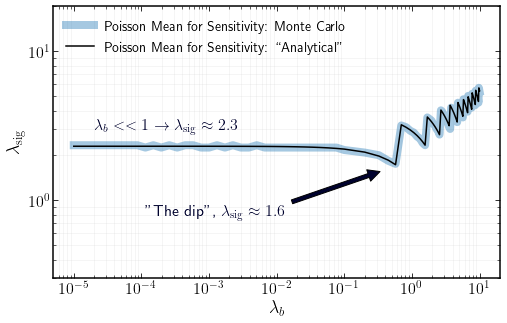
\includegraphics[width=0.53\textwidth]{figures/sensitivity_the_dip.png}
    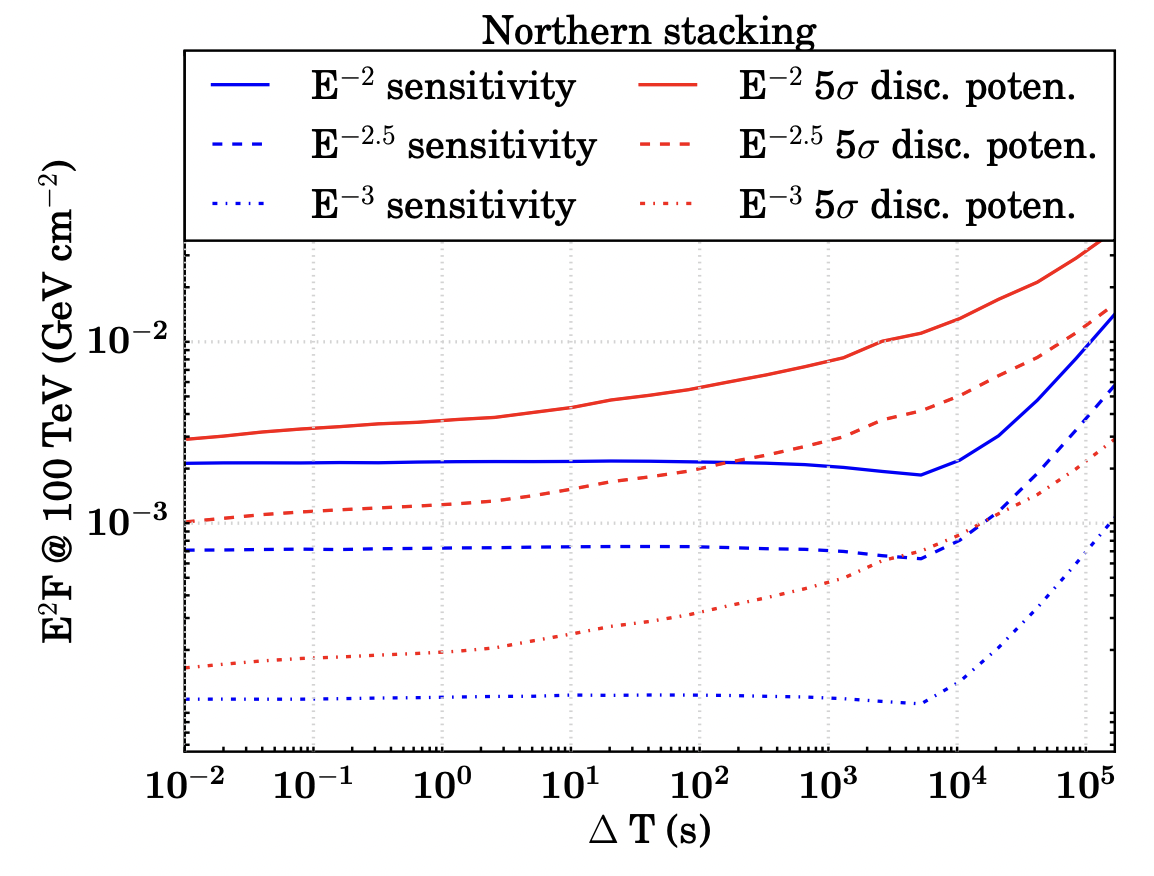
\includegraphics[width=0.46\textwidth]{figures/the_dip_icecube_example_frb.png}
    \caption{Sensitivity for a counting experiment (left) highlighting the location of ``the dip'' when the sensitivity seems to temporarily improve with increasing background. The blue line was calculated with a toy monte carlo and the black was calculated with Equation~\ref{eq:analytic}. The right hand figure shows a sensitivity plot from the 6 year FRB paper \cite{IceCube:2017fpg} where the dip is visible around $\Delta T = 10^4$~s.}
    \label{fig:sens_the_dip}
\end{figure}

Additionally, this is not just the case in toy counting experiment based analyses. This effect has shown up in many transient analyses in the past, because for short timescales, even with a likelihood construction, an analysis can essentially still behave as a counting experiment. In Figure~\ref{fig:sens_the_dip} we show in the left this for a toy counting experiment with $\lambda_b = \mathcal{R}\Delta T$. In the right, we show an example real IceCube analysis (with a likelihood approach), where this occurs as well. This effect, sometimes referred to as the ``sensitivity dip'' is also discussed in Sam Fahey's thesis (see Chapter 5 of \cite{samthesis}). The global minimum occurs when there the background expectation is slightly less than 0.5 events, and the corresponding sensitivity is approximately 1.6 events. 

\subsection{The ``flip-flop''}
Furthermore, in addition to the ``sensitivity'' of an analysis, we often quantify the discovery potential of analyses, which can also scale differently in these two regimes. The \textit{discovery potential} of an analysis is a quantity that is intimately related to the sensitivity, as methodologically it is calculated in a very similar manner. Whereas the sensitivity is the median 90\% CL upper-limit that would be placed under the assumption of the null hypothesis, the discovery potential for a certain spectral shape is defined as the flux normalization that would result in a specified significance at a certain fraction of trials.

This definition might seem vague, as ``specified significance'' and ``certain fraction'' were not clearly quantified. This is because the discovery potential can be calculated for different values of these parameters. For example, we can calculate both the $3\sigma$ and the $5\sigma$ discovery potential for the ``specified significance''\footnote{We will leave the discussion on the appropriateness of $3\sigma$ vs. $5\sigma$ discovery potentials up to someone else. It is my opinion that if it is computationally feasible to calculate $5\sigma$ or if you can validate that extrapolating a fit to your $\tsbg$ distribution is valid, then you should calculate $5\sigma$. If this is not the case, or if a plot is only meant to be shown internally, then $3\sigma$ is fine. In addition to considering wallclock time in computational considerations, I urge analyzers to also consider other impacts as well, see for example \cite{PortegiesZwart:2020pdu}}. In most background-dominated analyses, the convention for ``certain fraction'' is to use a 50\% CL, so for example a $3\sigma$ 50\% CL discovery potential is the signal strength that results in 50\% of trials that are at significant at least at the $3\sigma$ level, or
\begin{equation}
    q_{50}(\ts_{\mathrm{sig}}(\phi_0, \hat{\phi}(E))) > q_{99.7}(\tsbg) \; . 
\end{equation}

\begin{figure}
    \centering
    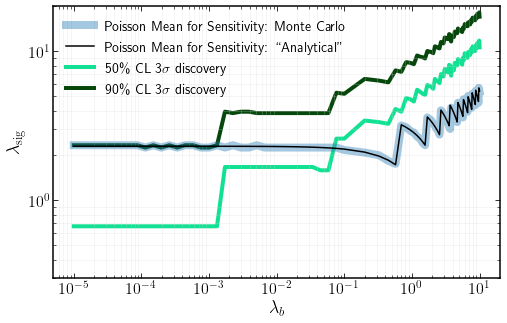
\includegraphics[width=0.5\textwidth]{figures/discovery_potential_flip_flop.png}
    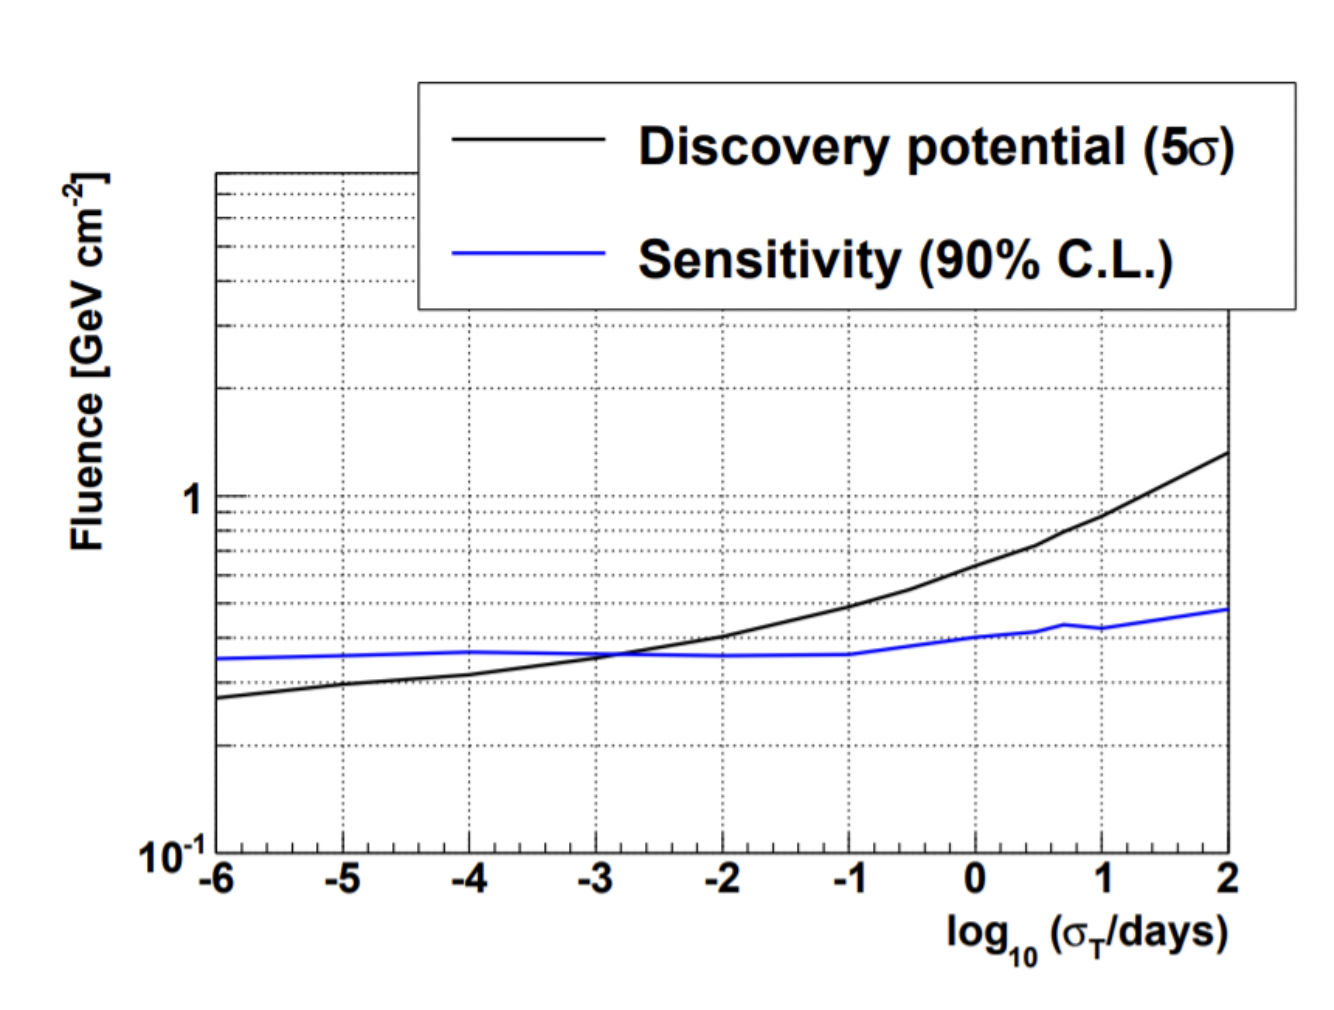
\includegraphics[width=0.49\textwidth]{figures/flare_flip_flop_example.png}
    \caption{Left: The same toy monte carlo as in Figure~\ref{fig:sens_the_dip}, but this time with the addition of $3\sigma$ discovery potentials with different confidence levels. The 50\% CL line (light green) is subject to the ``flip-flop'' between sensitivity and discovery potential, where the discovery potential is ``better'' than the sensitivity. When increasing the CL to match the one used for sensitivity, the discovery potential is always greater than or equal to the sensitivity. Right: an example analysis where the ``flip-flop'' is seen, taken from the all-sky flare analysis using 4 years of data \cite{IceCube:2015usw}.}
    \label{fig:flip_flop}
\end{figure}

However, for low background analyses, this common convention of using a 50\% CL for discovery potential can lead to counter-intuitive discovery potentials when compared to the sensitivity. Conventionally, it is the case that the discovery potential flux is larger than sensitivity flux, which is likely as anticipated because there should be a higher threshold for claiming discovery than for expected upper limits. In the case of low background analyses, we can have such a small background expectation, that even having a single background coincidence is significant. For the case of $3\sigma$, this is the same as saying when $q_{99.7}(\tsbg) = 0$. In this case, any coincident event satisfies both the threshold needed for sensitivity (comparing to the median) as well as for $3\sigma$ discovery. Then, the only thing that will determine the normalization of the discovery potential flux is the confidence level for the discovery potential, and if using a 50\% CL then you will need a smaller flux than that needed for the 90\% CL for sensitivity. In Figure~\ref{fig:flip_flop} we show in the left the different conventions for discovery potential confidence levels, and how the 50\% case can lead to this ``flip-flop'' between sensitivity and discovery potential, for a toy counting experiment. In the right, we show where this has shown up in previous IceCube analyses.

Our recommendation, moving forwards, is simply to explicitly define discovery potential when quoting it or showing it in a plot. If the analysis is in a regime where there might be the ``flip-flop,'' then it is up to their discretion to choose at which CL to define the discovery potential. There is precedent for either construction in previous IceCube papers.


\section{Discussion}
This note explored various conventions that we use when discussing or calculating various types of sensitivities or discovery potentials. All of the code needed to create the figures is provided on \href{https://github.com/apizzuto/flux_conventions}{Github}. Although we do not introduce any new techniques, we did show how some convention choices lead to confusion in understanding how our quoted sensitivities compare to model predictions. 

We summarize all of the major takeaways of the note below:
\begin{enumerate}
    \item Central energy ranges are informative for  sensitivities. The ``sensitivity'' and ``effective area'' construction for calculating these intervals answer slightly different questions, but are equivalent in some regimes.
    \item \vspace{-6pt} Always define your fluxes and sensitivities in terms of what they represent differentially, before calling something a ``fluence.'' If you want to use the word fluence, be explicit about whether this is a particle fluence scaled by $E^2$ or an energy fluence.
    \item \vspace{-6pt} When calculating differential sensitivities, be aware of how the choice of bin width affects the normalization within each bin (or use the construction that is independent of bin width).
    \item \vspace{-6pt} If comparing a differential sensitivity to a model, quantify the sensitivity to the model through a model rejection factor.
    \item \vspace{-6pt} Low background (ie short timescale) analyses have some features in sensitivities and discovery potentials that background-dominated analyses do not. Be mindful of ``the dip'' and ``the flip-flop.'' Neither of these effects are manifestations of anything incorrect, they are just a reflection of our convention choices. Define sensitivity and discovery potential explicitly to avoid confusion.
\end{enumerate}

\bibliographystyle{JHEP}
\bibliography{references}

\end{document}
